\section{Data analysis}
This section presents an analysis of the data gathered on the surveying test mission executed on the Odense model airfield
\subsection{Mission execution}
This subsection presents an analysis of data gathered of the mission executed, making emphasis on the study of flight precision characteristics such as flight height, flight path, side, and front overlap. 
\subsubsection{Flight path}
Using the data logging capabilities of the Apogee, its possible to reconstruct path traveled by the UAV.
Figure \ref{fig:SimVReal} shows a side by side comparison of the simulation and the real path flown by the UAV. The deviation on the flight its caused by the wind. The effect of the wind on the aircraft capability to follow the design path can have a significant impact on the success of the mission, especially since the fixed-wing UAV cannot hover or fly backward. 
\begin{figure}[H]
\centering
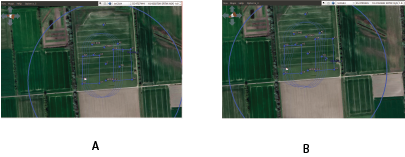
\includegraphics[width=16cm,height=16cm,keepaspectratio]{imagenes/SimVsreallity.png}
\caption{ A: Simulation of surveying mission. B: Surveying mission execution}
\label{fig:SimVReal}
\end{figure}
Using the geolocation of each picture is possible to recreate the UAV path. Figure n shows a line plot of the position of each photo.
\begin{figure}[H]
\centering
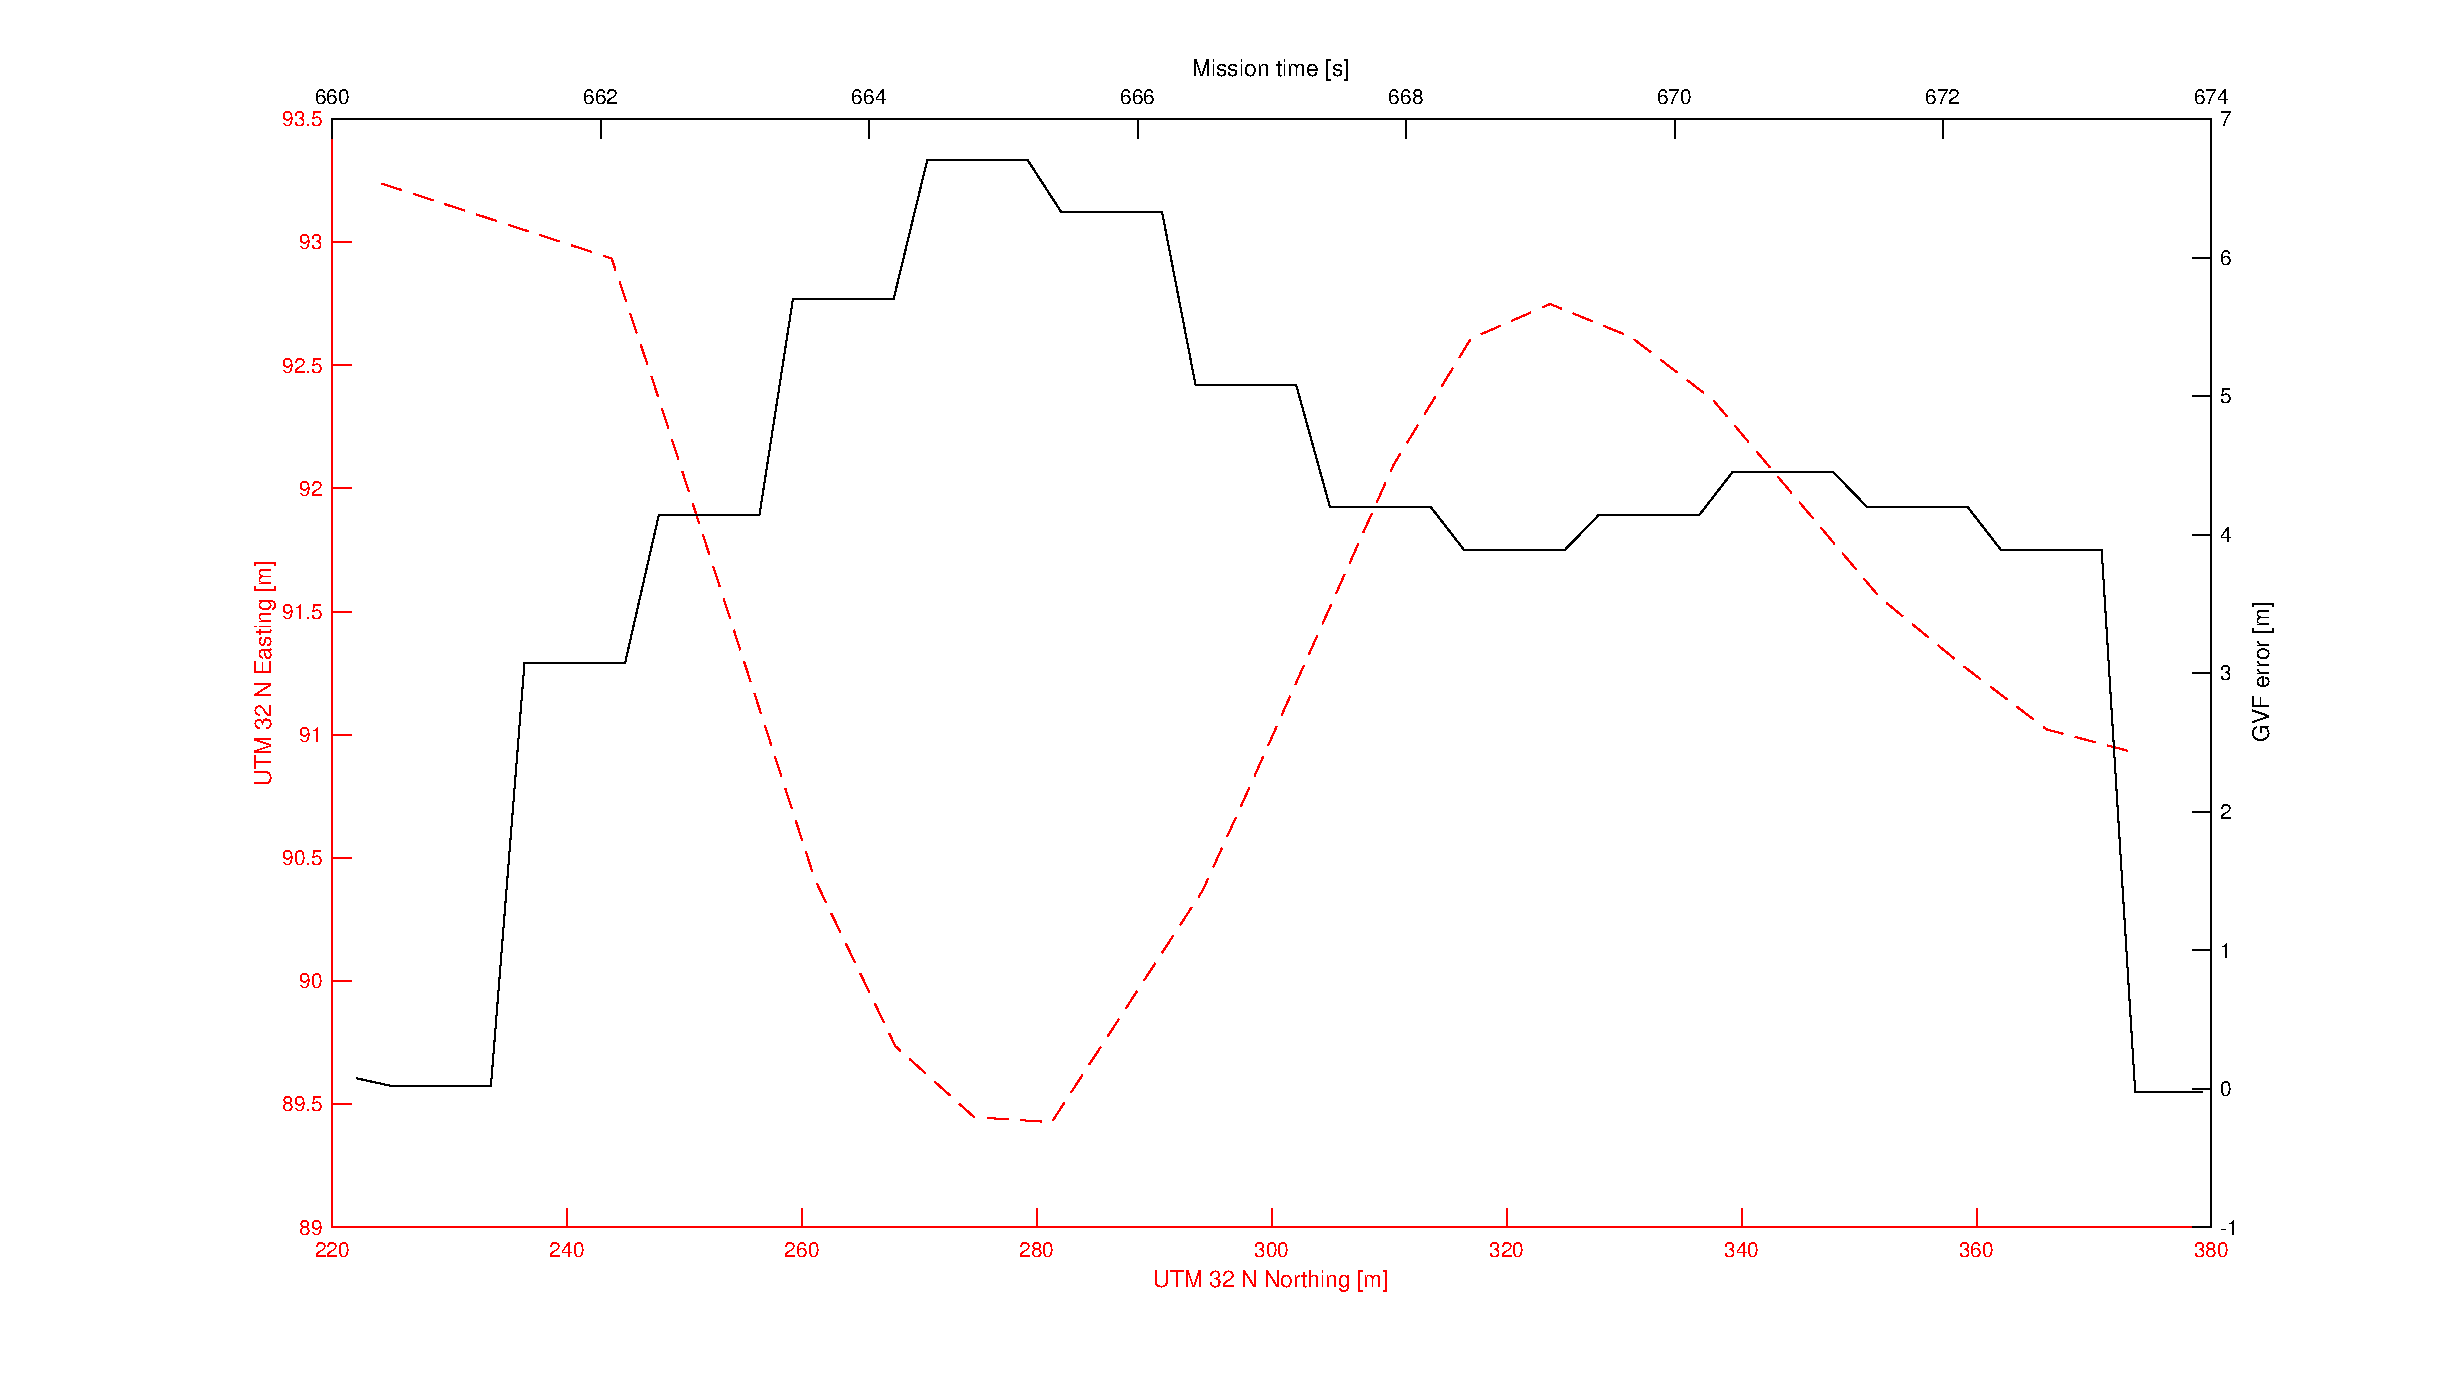
\includegraphics[width=16cm,height=16cm,keepaspectratio]{imagenes/graph.eps}
\caption{ Flight path line plot for surveying mission of field B}
\label{fig:FielB}
\end{figure}
\subsection{Front and side overlap}
When designing surveying mission flight path, two of the main criteria used are side and front overlap, these together with GSD are use to compute the distance between photos and distances between strips. These distances are the input for the navigation algorithm in charged of the navigation.
\subsubsection{Front overlap}
The front overlap is closely related to the distance between consecutive photos in the same path strip.  Using the geolocation of each photography is possible to find the distance traveled by the UAV between each picture. The spacing between the images should be 7.2 m, taking into consideration the error associated with GPS measurements of +- 4m. 

\begin{table}[H]
\centering
\begin{tabular}{|c|c|l|c|l|c|l|c|c|}
\hline
 & \multicolumn{8}{c|}{Number of photo in a X range of meters}                                                                                                                            \\ \hline
Surveying field         & \multicolumn{2}{c|}{X \textless 3.2} & \multicolumn{2}{c|}{3.2 \textless X \textgreater 11.2} & \multicolumn{2}{c|}{X \textgreater 11.2} & Turning points & Total                      \\ \hline
A                       & 6               & 5 \%               & 95                        & 81 \%                      & 17                 & 14\%                & 8              & 126                        \\ \hline
B                       & 3               & 2 \%                & 109                       & 79 \%                      & 26                 & 19\%                & 9              &  147 \\ \hline
\end{tabular}
\caption{Result of front overlap test}
\label{Table:FrontOverlap} 
\end{table}
\subsection{Side overlap}
The side overlap is closely related to the distance between consecutive strip.  Using the geolocation of each photography is possible to . The spacing between the images should be 7.2 m, taking into consideration the error associated with GPS measurements of +- 4m. 

\subsection{Photogrammetric products}
The image alignment, dense point cloud, and DEM construction were done using Agisoft Photo Scan Pro, and the results of the image processing procedure are shown in images \ref{fig:ResultBprocessing}, table \ref{Table:ResultsB} shown a more comprehensive data analysis of the different parameters of the mission.
\begin{figure}[H]
\centering
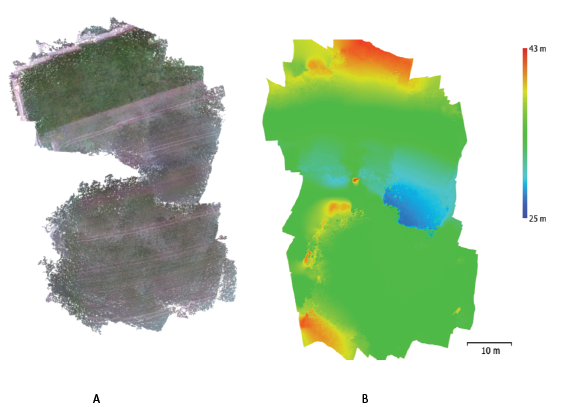
\includegraphics[width=16cm,height=16cm,keepaspectratio]{imagenes/ResutsB.png}
\caption{ A: Orthomosaic field B B: DEM field B}
\label{fig:ResultBprocessing}
\end{figure}

\begin{table}[H]
\centering
\begin{tabular}{|c|c|c|c|}
\hline
Surveying mission field B & Simulation & Experimental & Error (\%) \\ \hline
Fotos align               & -          & 147/147      & 0          \\ \hline
Altitude reported (m)     & 50         & 21.3         & 57.4       \\ \hline
GSD (cm/pixel)            & 1.33       & 3.5          & 62.2       \\ \hline
Coverage area (m2)        & 24000      & 7875         & 69.5       \\ \hline
\end{tabular}
\caption{Result of surveying mission over field B}
\label{Table:ResultsB}
\end{table}
Analyzing the data obtained from the software, is notable the error associated with the photogrammetric product are important. Although all the images were aligned, this process was not done correctly. Figure n shows an example of the error made by the alignment algorithm. 

There are several factors to take into consideration to explain the reasons for this behavior: the most important one: the Around 95 \% of pictures present \textit{vignetting}. Vignetting refers to the phenomenon of brightness attenuation away from the image center, and is an artifact that is prevalent in photography. Although not objectionable to the average viewer, it can significantly impair computer vision algorithms that rely on precise intensity data to analyze a scene. Applications in which vignetting distortions can be particularly damaging include photometric methods such as shape from shading, appearance-based techniques such as object recognition, and image mosaicing.  Figure \ref{fig:vignetting} shows a picture with vignetting.\cite{4663074}

\begin{figure}[H]
\centering
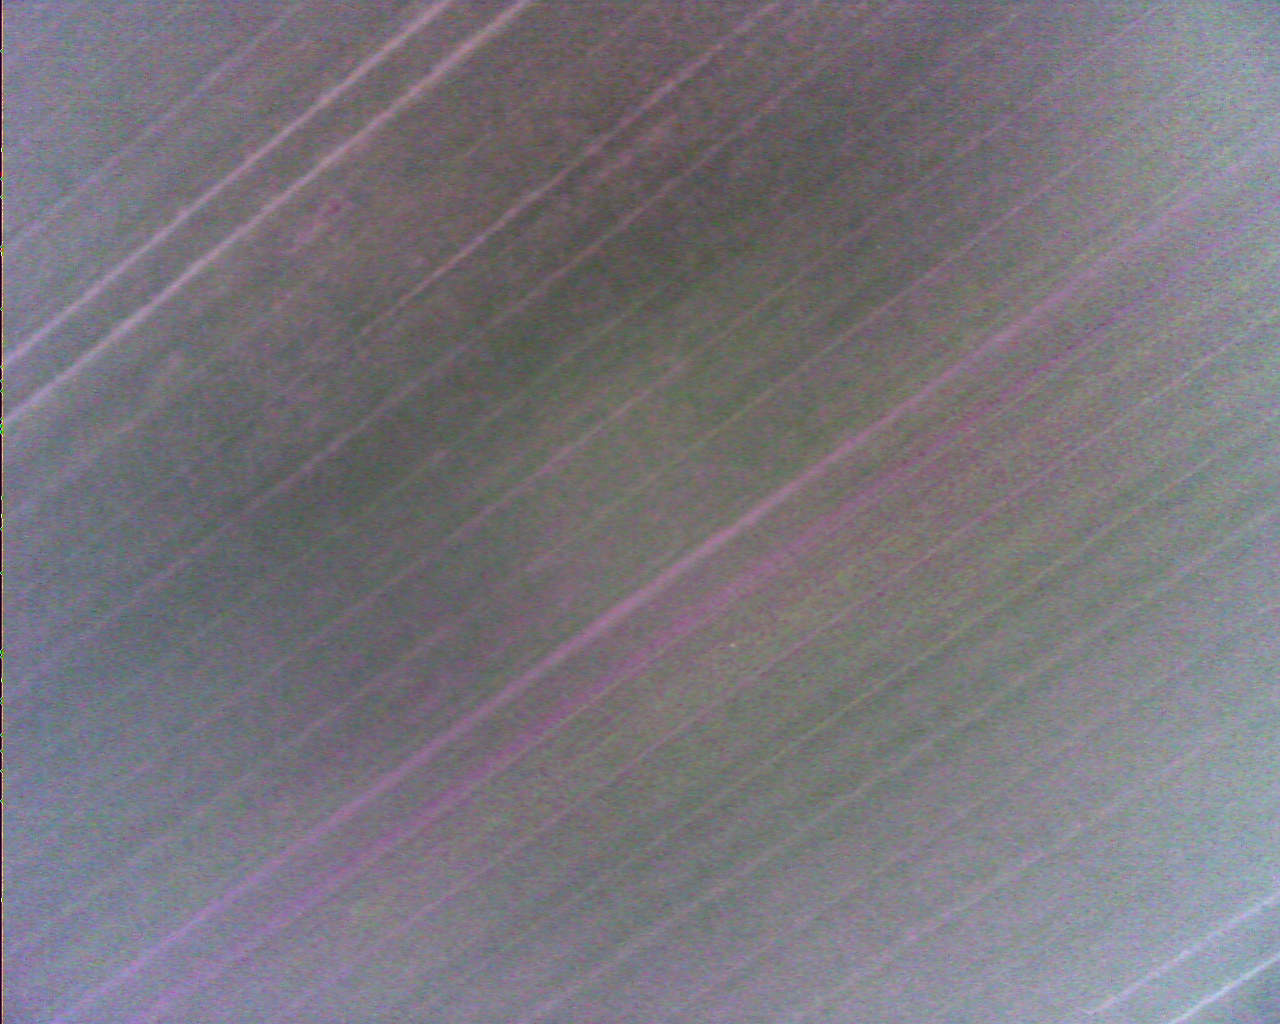
\includegraphics[width=16cm,height=16cm,keepaspectratio]{imagenes/IMG_62.png}
\caption{Picture with vignetting from the surveying mission}
\label{fig:vignetting}
\end{figure}
Table \ref{Talbe:XYerror} show the error of camera location estimator algorithm. taking into consideration that the field has a dimension of $X = 75 m and Y = 105 m$
\begin{table}[H]
\centering
\begin{tabular}{|c|c|c|}
\hline
   & \multicolumn{2}{c|}{Camera location estimation error} \\ \hline
   & Meters                     & \%                       \\ \hline
x  & 40.89                      & 45.3                     \\ \hline
Y  & 41.57                      & 60.3                     \\ \hline
XY & 58.31                      & --                       \\ \hline
\end{tabular}
\caption{Average camera location error}
\label{Talbe:XYerror}
\end{table}